(20 marks) For Catmull-Clark subdivision, we would like to subdivide only a particular area
of the mesh using an adaptive subdivision method.
\begin{enumerate}
\item Extend the simple (naive) T-junction insertion method of Adaptive Loop subdivision to create an Adaptive Catmull-Clark subdivision. Draw a figure to support your description. \\
Note: the picture is taken from the CPSC589 notes, page 126. \\
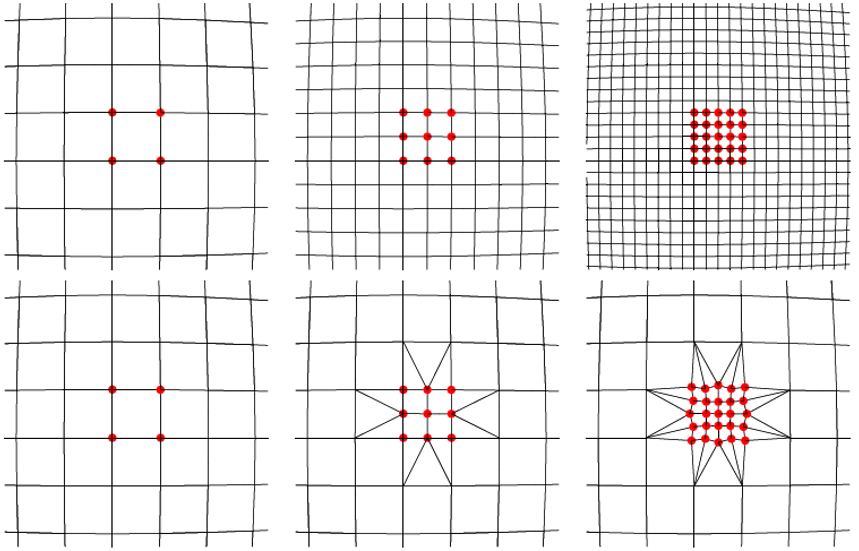
\includegraphics[width=400bp]{q6_pic.png} \\
To make a local subdivision via Catmull-Clark, a simple method is to perform Catmull-Clark, as normal in the local area, but then modify the immediately surrounding barrier to fill-in the gaps of the new edge-vertexes (gaps exist if it is not perfectly flat). \\
To do this, we have to add two edges, (instead of 1 for loop), connecting the new mid-edge point, to the two closest vertices outside the subdivided area. \\
(Note: This is only true for the first subdivision, after this they're triangles, and use the same T-junctions for smoothing to the un-divided area)\\

\item Describe the disadvantages of this simple adaptive subdivision. \\
It creates a lot of 'long' triangle, as it repeatedly subdivides. \\
It also ends up creating a high difference-of-detail on some vertices. Ex: on the far-right of the picture, the surrounding vertices, some edges go to vertices with valence 4, while some goto vertices with valence 7. This also implies that these are no longer regular. \\

%This will also make these shapes extra-oridnary for global subdivisions?
\end{enumerate}
